% ---------------------------------------------------------------------------
% Appendix: Model and Temperature Ablations + the Frontier Tier (v3).
% Adapted from v2 appendix_ablations. Per the revision directive:
% third-price and common-value (winner's-curse) rows/prose REMOVED from all
% tables (full batteries remain in the replication package); the frontier
% "constraints migrate via TPSB" argument is cut with the format and replaced
% by the registered +X unfamiliar-format probe; refs retargeted to v3 labels
% (app:cardinal for the tuning grid; sec:map for the design map).
% NOTE for co-authors: v2's TPSB-based evidence that frontier reasoning fails
% non-textbook formats (gpt-5-mini SMAD 60% at n=3) is no longer in the paper;
% its scope role is reassigned to the pending 2P+X/AC+X battery (E-v3-1).
% ---------------------------------------------------------------------------
\section{Model and Temperature Ablations, and the Frontier Tier}\label{app:ablations}

This appendix reports the stability ablations referenced in Section~\ref{sec:validation}---varying the sampling temperature of the GPT-4o anchor, and varying the base model on the fidelity battery---together with the two robustness tiers that bound the panel's regime: a capability floor (Llama-3-8B) and a frontier tier (gpt-5-mini, gpt-5, Claude Sonnet 5, Gemini 2.5 Flash) on which the full lever grid was run. Throughout, the human column is the moment-matched reconstruction of Section~\ref{sec:reconstruction}; consistent with the epistemic policy stated there, we report \emph{no} significance tests against reconstructed human benchmarks. Comparisons to the human column should be read qualitatively---rankings, directions, and orders of magnitude. \TODO{Attach Monte-Carlo percentile bands (and, once available, the parametric-bootstrap bands of Appendix~\ref{app:human}) to the human column in both tables (plan \S 5.8).}

\subsection{Varying temperature for the GPT-4o agent}

We vary GPT-4o's sampling temperature $T \in \{0.1, 0.5, 1.0\}$ across the fidelity-battery formats (Table~\ref{tab:temperature}; Figure~\ref{fig:ablations-temperature}). Two facts stand out. First, temperature effects are modest and, crucially, \emph{non-monotonic}: no temperature setting dominates. Within the paper's scope, $T=0.1$ is strictly best in the two ascending-clock formats---near-deterministic decoding removes stochastic exits from an already-truthful modal policy, driving SMAD to exactly $0.00$---and strictly worst in all three sealed-bid formats, where the same determinism locks in the modal bias. Second, the pattern is consistent with temperature scaling the dispersion around the model's modal action rather than changing the underlying strategy. We therefore retain $T=0.5$ throughout the paper as a \emph{convention}---it is the most common setting in LLM-based simulation \citep{horton2023large} and preserves comparability across models and with prior work---not because it is performance-optimal in any format. Temperature reappears in Appendix~\ref{app:cardinal} as a candidate knob for \emph{cardinal} calibration to human levels; its effects there are likewise non-monotonic (on the rebuilt grid's normalization, SPSB-IPV SMAD is $15.1/8.9/13.2$ at $T=0.1/0.5/1.0$).

\begin{figure}[H]
    \centering
    
\includegraphics[scale=0.35]{appendix2_temperature_comparison.png}
    \caption{Comparison of the bidding behavior of reconstructed human participants and GPT-4o across three temperature settings ($T=0.1, 0.5, 1.0$). The horizontal bars represent the scaled mean absolute deviation (SMAD) from the theoretical benchmark, with error bars indicating 95\% confidence intervals (for the LLM cells only; see the text of this appendix for the human column's epistemic status). \TODO{Regenerate the asset restricted to the five in-scope formats (the current PNG includes two out-of-scope common-value panels).}}
    \label{fig:ablations-temperature}
\end{figure}

\begin{table}[htbp]
\centering
\begin{tabular}{l|ccc}
\hline
Auction Format & $T=0.1$ & $T=0.5$ & $T=1.0$ \\
\hline
AC-B (closed clock), APV & 0.00 & 0.47 & 2.15 \\
AC (open clock), APV & 0.00 & 0.81 & 1.00 \\
SPSB, IPV & 14.77 & 8.69 & 12.89 \\
SPSB, APV & 12.87 & 10.73 & 12.75 \\
FPSB, IPV & 28.07 & 27.55 & 24.99 \\
\hline
\end{tabular}
\caption{Temperature effects on GPT-4o bidding behavior (SMAD, \%), in-scope formats. SMAD = scaled mean absolute deviation from the theoretical benchmark. No temperature dominates: $T=0.1$ is strictly best in the two clock formats and strictly worst in the three sealed-bid formats. Values use the legacy figure normalization ($\mathbb{E}[b^\star]=25$); the rebuilt cell-level grid normalizes by $24.5$, making values uniformly $\approx 2\%$ larger (e.g., SPSB-IPV $15.1/8.9/13.2$)---orderings and the non-monotonicity are unaffected. The out-of-scope common-value rows of the legacy battery remain in the replication package.}
\label{tab:temperature}
\end{table}

\subsection{Varying the base model}

We repeat the fidelity battery, holding prompts fixed and $T=0.5$, for three models beyond the GPT-4o anchor: Claude 3.5 Haiku, Gemini 2.0 Flash, and Llama-3-8B-Instruct (an open-weight model).\footnote{Model identifiers: \texttt{claude-3-5-haiku-20241022}, \texttt{gemini-2.0-flash}, \texttt{Meta-Llama-3-8B-Instruct}, and, in the frontier tier below, \texttt{gpt-5-mini}, \texttt{gpt-5}, \texttt{claude-sonnet-5}, and \texttt{gemini-2.5-flash}. An earlier draft referred to the Anthropic model as ``Claude Sonnet 3.5''; the experiment configurations confirm that the runs stored under directories named \texttt{claude\_sonnet} were in fact executed with \texttt{claude-3-5-haiku-20241022} (config-verified: \texttt{configs/clock/01\_06\_ascending\_clock\_apv\_claude\_sonnet.yaml}). The gpt-5-mini API ignores the temperature parameter.} Claude 3.5 Haiku and Gemini 2.0 Flash belong to the panel of Section~\ref{sec:design}; Llama-3-8B-Instruct and the frontier tier of Section~\ref{app:ablations-frontier} bracket the panel from below and above. Results appear in Table~\ref{tab:models} and Figure~\ref{fig:ablations-models}. The fourth panel member, Gemma 27B, ran a separate sealed-bid fidelity battery (Table~\ref{tab:gemma-fidelity}); we report it apart from Table~\ref{tab:models} because its cells are recomputed from the cell-level dataset (\path{results/merged_ranking/auction_cells.csv}, normalizer $\mathbb{E}[b^\star]=24.5$), a normalization that differs from the legacy figure scaling of the Claude/Gemini/Llama columns here (the same $\approx\!2\%$ offset flagged for Table~\ref{tab:temperature}), so the columns are not directly comparable cell-for-cell.

Llama-3-8B-Instruct serves as the \emph{capability floor}. It exhibits substantially degraded performance across all auction formats (mean SMAD $57.58\%$ over the legacy seven-format battery, exceeding the reconstructed human benchmark in six of seven formats)---evidence that open-weight availability at small scale is not sufficient for competent strategic play, and that the panel models sit well inside the band where design levers have room to operate. Claude 3.5 Haiku and Gemini 2.0 Flash behave broadly like the GPT-4o anchor: near-truthful in the clock formats and moderate deviations in the sealed-bid formats. \TODO{The SPSB-IPV cells will be recomputed on the harmonized canonical dataset alongside signed means (plan E8, \S 5.3).} \TODO{Regenerate the figure asset \texttt{appendix2\_model\_comparison.png}: the legend of the current PNG carries the superseded ``Claude Sonnet 3.5'' label, its gpt-5-mini series rests on the misattributed logs documented in Section~\ref{app:ablations-frontier} and must be dropped or rebuilt from the genuine cells, and the out-of-scope common-value panels should be removed.}

\paragraph{Gemma 27B and the difficulty ordering.}
The open-weight Gemma 27B model ran the sealed-bid fidelity battery ($K=30$ per cell; the in-scope rows appear in Table~\ref{tab:gemma-fidelity}; across its full legacy six-format battery its mean SMAD is $19.09\%$, between the panel models and the Llama floor). The instructive fact is not the level but the \emph{shape}: Gemma does \emph{not} reproduce the human difficulty ordering cleanly. In the human data the first-price format is much harder than the second-price dominant-strategy format---FPSB-IPV SMAD $24.76\%$ versus SPSB-IPV $5.65\%$, a ratio of $4.4$---and GPT-4o preserves that ordering ($27.55\%/8.69\% = 3.2$). Gemma nearly flattens it: $24.80\%$ in FPSB-IPV against $19.88\%$ in SPSB-IPV, a ratio of only $1.25$. It deviates almost as much in the format where truthful bidding is dominant as in the format where equilibrium requires shading, so the human-like difficulty \emph{spacing} that the anchor model displays is itself partly model-specific---a fact the validity map records (Section~\ref{sec:validation-map}) and the ordinal table reports as attenuation (Table~\ref{tab:ordinal}). The two ascending-clock cells are not yet run for Gemma in the fidelity battery (the per-tick clock harness is slow, and reconciling the survey-style elicitation with the tick protocol is deferred to the native-key runs); Gemma's design-map clock cell (Section~\ref{sec:map-extensive}) is a separate, completed run. \TODO{Gemma fidelity-battery ascending-clock (AC and AC-B) cells pending native-key runs; survey-vs-tick harmonization deferred.}

\begin{table}[htbp]
\centering
\footnotesize
\begin{tabular}{l c c}
\hline
Auction Format & SMAD vs.\ value (\%) & Signed mean dev.\ (\$) \\
\hline
FPSB, IPV & 24.80 & $-5.89$ \\
SPSB, IPV & 19.88 & $-4.87$ \\
SPSB, APV & 18.67 & $-4.57$ \\
\hline
\end{tabular}
\caption{Gemma 27B sealed-bid fidelity battery, in-scope formats (SMAD, \% of $\mathbb{E}[b^\star]=24.5$; signed mean deviation from value in dollars). Recomputed from \texttt{results/merged\_ranking/auction\_cells.csv} (group \texttt{gemma27b}, $K=30$ per cell). Gemma's FPSB-IPV/SPSB-IPV ratio is $1.25$, against $4.4$ for reconstructed humans and $3.2$ for GPT-4o: the model preserves the direction of the difficulty ordering but not its spacing. Out-of-scope rows of the legacy battery remain in the replication package.}
\label{tab:gemma-fidelity}
\end{table}

\begin{figure}[H]
    \centering
    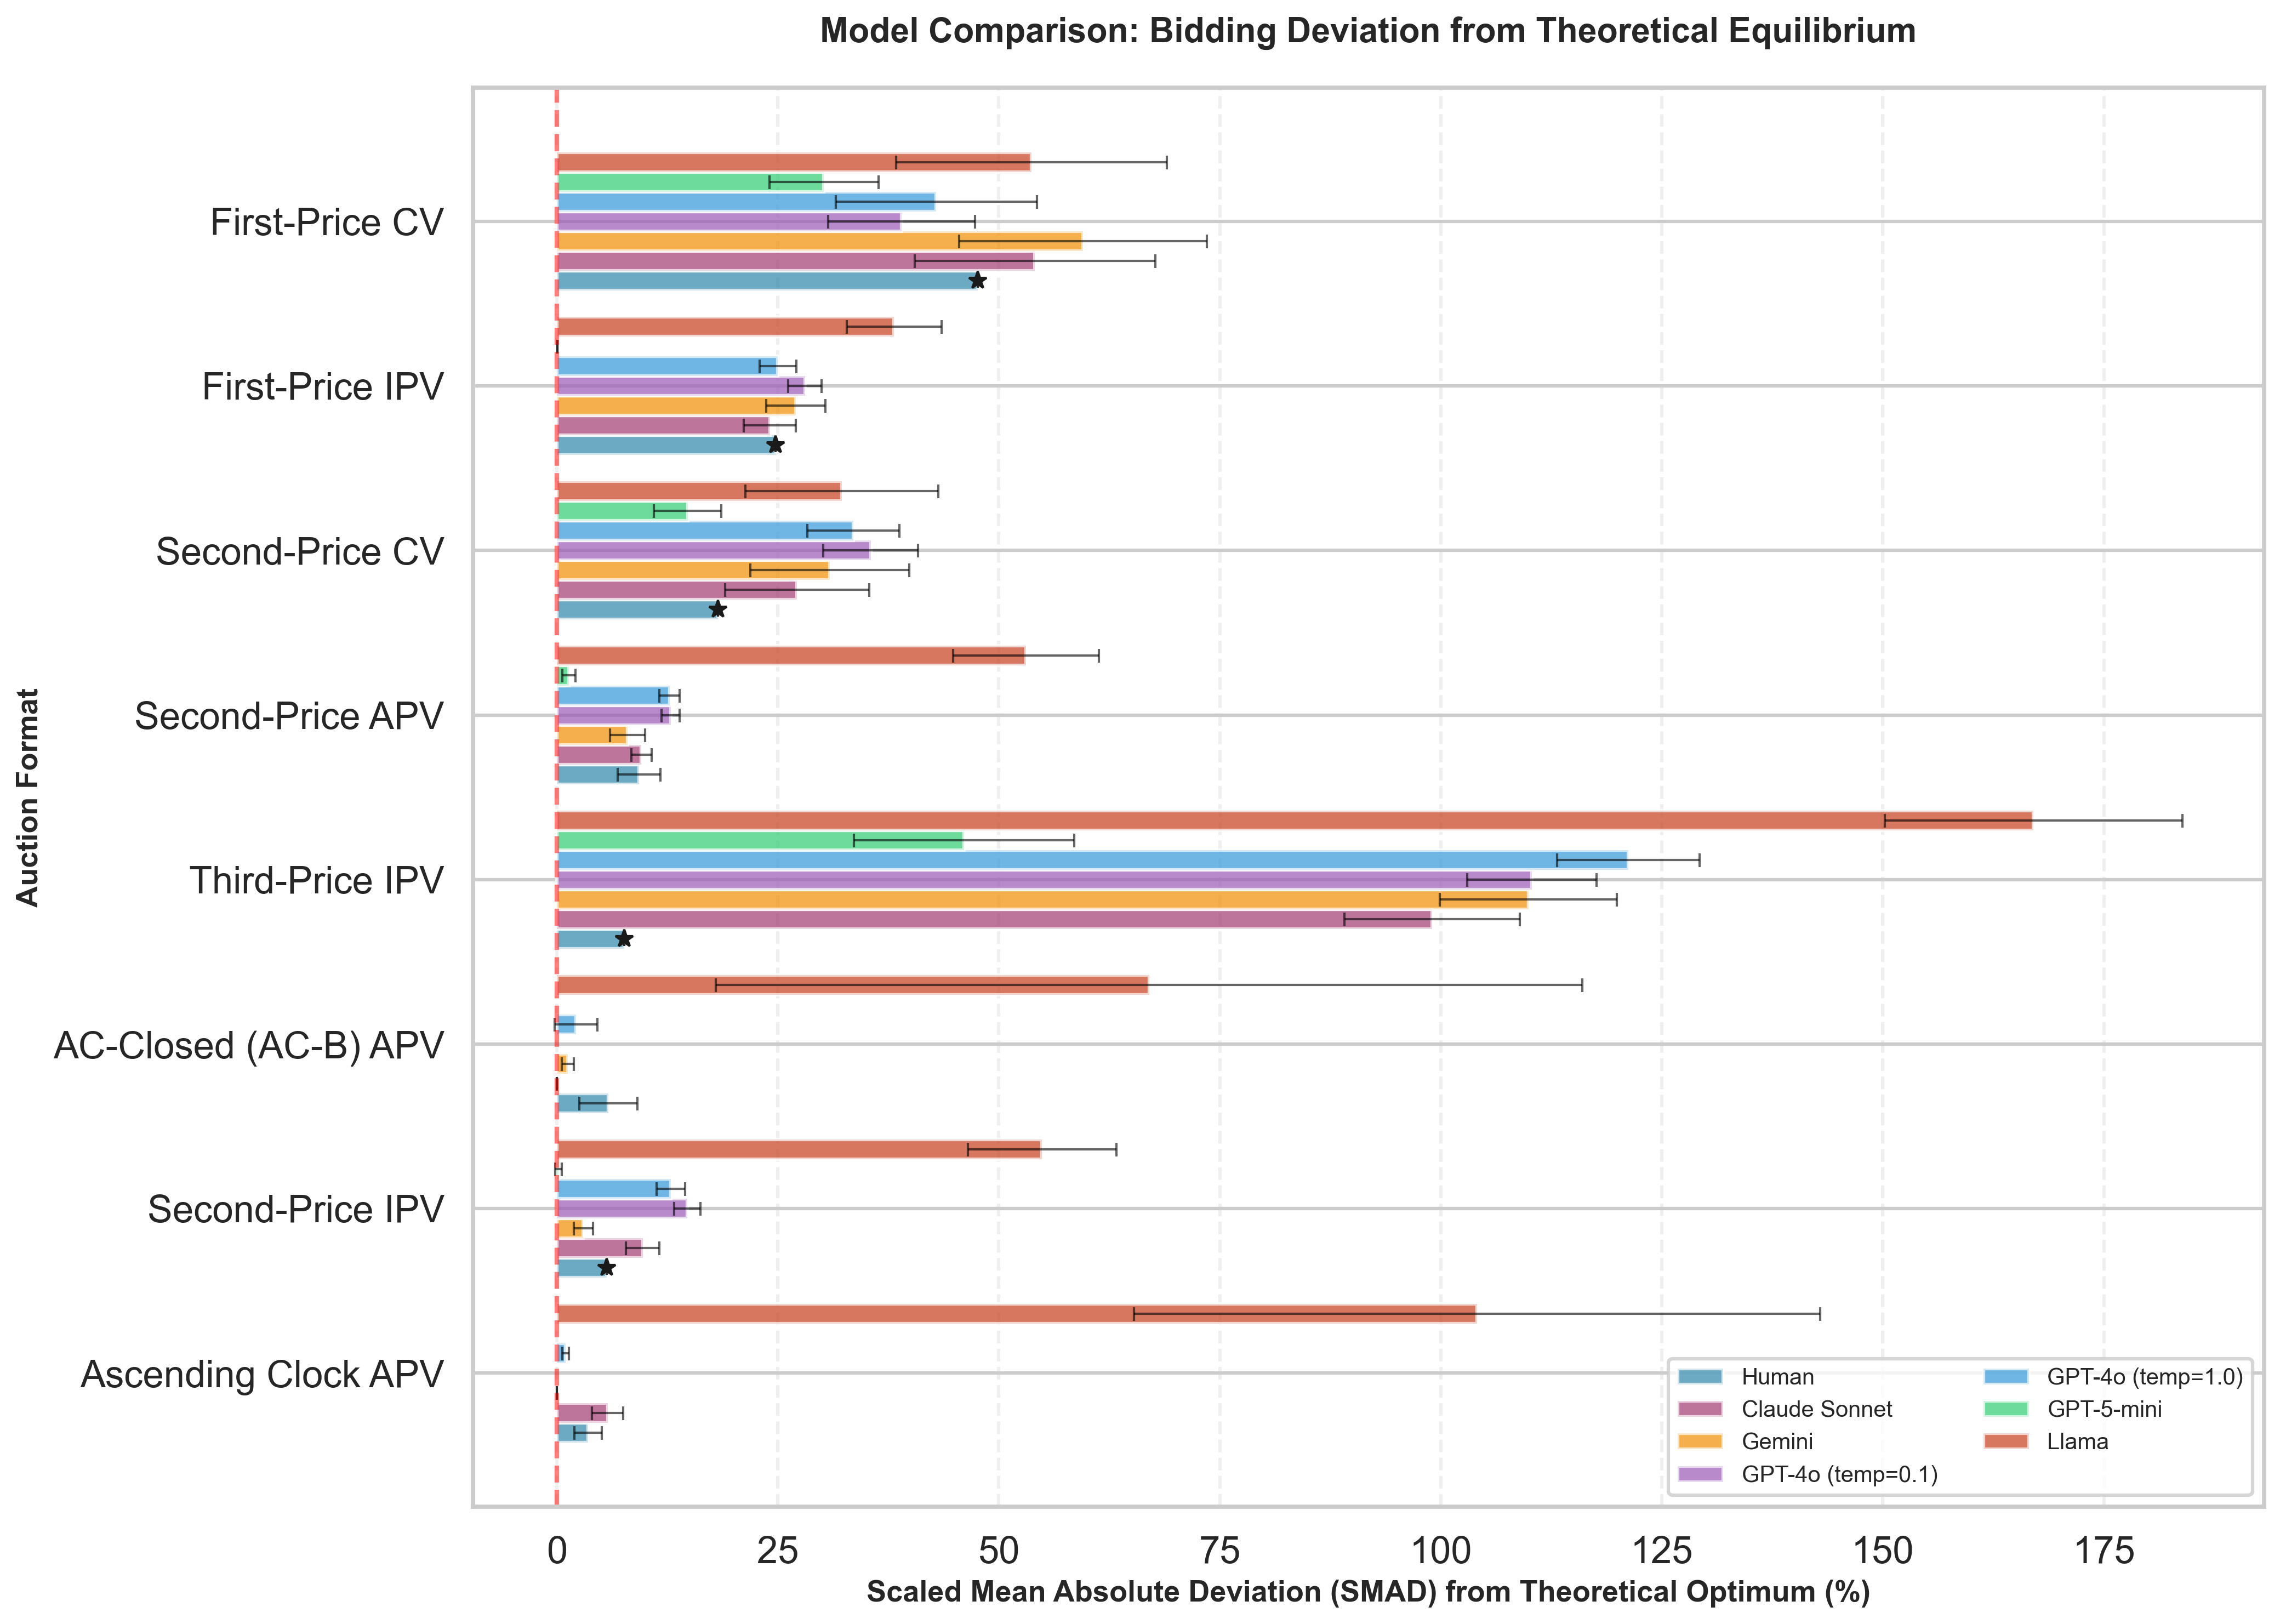
\includegraphics[scale=0.375]{appendix2_model_comparison.png}
    \caption{Comparison of the bidding behavior of reconstructed human participants and LLM agents across further foundation models. The horizontal bars represent the scaled mean absolute deviation (SMAD) from the theoretical benchmark, with error bars indicating 95\% confidence intervals (LLM cells only). The gpt-5-mini series shown in the current asset is superseded (see the frontier discussion in the text; regeneration pending, together with removal of the out-of-scope panels).}
    \label{fig:ablations-models}
\end{figure}

\begin{table}[htbp]
\centering
\begin{tabular}{l|c|ccc}
\hline
\multirow{2}{*}{Auction Format} & Human & Claude 3.5 & Gemini 2.0 & Llama-3-8B \\
 & (reconstr.) & Haiku & Flash & \\
\hline
FPSB, IPV & 24.76 & 24.09 & 27.05 & 38.16 \\
SPSB, IPV & 5.65 & 9.72 & 3.01 & 54.89 \\
AC-B (closed clock), APV & 5.83 & 0.00 & 1.26 & 67.00 \\
SPSB, APV & 9.31 & 9.58 & 8.02 & 53.08 \\
AC (open clock), APV & 3.54 & 5.74 & 0.00 & 104.10 \\
\hline
\end{tabular}
\caption{Fidelity battery across base models, in-scope formats (SMAD, \%). All models run at $T=0.5$. The human column is the moment-matched reconstruction of Section~\ref{sec:reconstruction}; no significance tests are reported against it because the reconstruction is model-based (see text and Appendix~\ref{app:human}). An earlier draft's gpt-5-mini column is removed: its source logs are GPT-4o (see the frontier subsection); the genuine gpt-5-mini cells appear in Table~\ref{tab:ablations-frontier}. Out-of-scope common-value rows remain in the replication package.}
\label{tab:models}
\end{table}

\subsection{The frontier tier: truthful at baseline, still breakable by presentation}\label{app:ablations-frontier}

An earlier draft treated gpt-5-mini as a frontier \emph{ceiling} that plays near-optimally across a battery of sealed cells (mean SMAD $6.68\%$). That figure did not survive a provenance audit: the log tree from which it was computed (\path{recovered_logs/experiment_logs_with_explanation/V10/}) is GPT-4o in every run configuration---not gpt-5-mini---and shares most of its run identifiers with the anchor logs, so it is discarded; the $6.68\%$ figure is retired, not merely re-sourced. Two data sources replace it. First, a genuine gpt-5-mini sealed-bid battery (Table~\ref{tab:ablations-frontier}, in-scope rows). Second, a full intervention grid run on four frontier models---gpt-5-mini, gpt-5, claude-sonnet-5, and gemini-2.5-flash (canonical identifiers; family \texttt{es\_v12} in \path{results/merged_ranking/auction_cells.csv})---reported in Table~\ref{tab:frontier-grid}. (The formerly empty gpt-5-mini clock cells are explained: a configuration typo, \path{configs/clock/01_07_ascending_clock_apv_closed_gpt5mini.yaml} carrying the invalid model id \texttt{gpt-4-mini}, suppressed the runs; with the typo fixed, a genuine gpt-5-mini clock cell exists, $K=50$, SMAD $1.25\%$.)

\paragraph{Baselines: the map's positive cells have nothing left to do.}
In the dominant-strategy formats the frontier tier is essentially perfect out of the box. gpt-5-mini's mean deviation is $-\$0.05$ (SMAD $0.2\%$) in SPSB-IPV and $-\$0.34$ ($1.4\%$) in SPSB-APV---truthful play at levels the panel models reach only under the strongest levers---and in FPSB-IPV its bids sit $\$8.53$ below value on average, i.e., almost exactly on the risk-neutral equilibrium shading rule $\frac{n-1}{n}v$ (mean deviation from the RNE benchmark $+\$0.002$; SMAD against RNE $0.1\%$): it applies the textbook formula.\footnote{The cell-level data report deviations against both truthful bidding and each format's own equilibrium benchmark; against truthful bidding the FPSB cell reads SMAD $34.8\%$, which measures correct equilibrium shading, not error.} Across the frontier grid (Table~\ref{tab:frontier-grid}), all four models are essentially exactly truthful at every sealed baseline (mean deviations $0.00$--$0.30$; SMAD $0$--$2.3\%$), and the safety, payoff-tree, second-order-belief, and clock-framing description cells are inert---they land on the same $\approx 0$ play, because no baseline error remains to move. This is the compression the main text's scope statement reports (Section~\ref{sec:discussion-scope}): the design map's positive cells are levers for the bounded-rationality regime, and the frontier tier has exited that regime in the formats we measure. Whether unfamiliar strategy-proof formats reopen it is the registered +X question. \TODO{Run the 2P+X / AC+X battery on both the panel and the frontier tier (E-v3-1); the predecessor draft's evidence on this point used the third-price format, which is outside the current scope.}

\paragraph{The backfire cells keep their teeth: retrieval selection.}
Presentation, however, still breaks frontier models---through a failure mode with a different signature than the panel's. (i) \emph{The menu restatement} collapses claude-sonnet-5 from exact truthfulness to a mean deviation of $-\$8.71$ (SMAD $35.5\%$, Cohen's $d=-3.8$, $p<10^{-58}$) and degrades gemini-2.5-flash (SMAD $2.3\% \to 9.1\%$, $p<10^{-8}$), while leaving gpt-5 and gpt-5-mini exactly truthful---the same sign-mixed, model-specific pattern as the panel's menu cell (Appendix~\ref{app:heterogeneity}), now with one model driven to a $35\%$ deviation. The traces say exactly what broke: under the menu wording, claude-sonnet-5 announces that ``the standard first-price auction equilibrium bid is $(n-1)/n$ of my value'' and executes that formula flawlessly---its $-\$8.71$ is almost exactly the $-\tfrac{1}{3}\,\mathbb{E}[v] \approx -\$8.17$ the first-price rule implies---despite the prompt stating that the winner pays the highest \emph{rival} bid. The unfamiliar wording did not degrade play into noise; it re-classified the game and retrieved the wrong textbook solution, executed perfectly. (ii) \emph{What looks like a clock inversion is the same failure}: relative to its near-perfect sealed play, the legacy closed clock raises claude-sonnet-5 to SMAD $8.6\%$, with $75\%$ of exits more than a dollar early---but the legacy clock cells carry an affiliated-values \emph{description}, and the model's exit rationales explicitly invoke the winner's curse (``others' persistence signals possibly similar high values, risking overpayment''), a script correct in common-value clocks and inapplicable here, where the bidder knows its own value. A clean IPV-described rerun of the same cell restores near-perfect play: SMAD $2.0\%$, early exits $3\%$, marginal-reasoning traces (``price equals my value; drop''). One sentence of affiliation language costs an otherwise exactly-truthful model eight SMAD points by activating the wrong playbook---while the same sentence leaves the panel models' clock gains intact, because they have no winner's-curse script to misfire. gpt-5 ($+\$0.61$) and gpt-5-mini ($+\$0.28$) shift only by roughly the \$0.5 tick granularity, with clean marginal reasoning throughout.

The gpt-5 cells carry reduced and uneven $K$: the model frequently omits the required response tags, and unparseable repetitions are dropped, so per-cell $n$ (in bids) ranges from $15$ to $150$ ($102$ for the SPSB baseline after its final top-up); read the $n$ column as a sample-size caveat; the run set is frozen. \TODO{gpt-5 intervention cells: top up and re-freeze $n$ before the final draft; runbook at \path{plan/FRONTIER_RUNBOOK.md}.}

\paragraph{Implication for the main text.}
The frontier tier sharpens the paper's scope condition into an asymmetric rule. On one side, the simplifying levers are (at worst) wasted on frontier agents: with no baseline error to preserve, the preservation index is undefined and the positive cells are inert. On the other, presentation choices still carry real risk---a description with no incentive content can break an otherwise perfect strategic reasoner, and \emph{which} reasoner it breaks is not predictable from baseline capability---so the practitioner guidance of Section~\ref{sec:discussion} (expose invariants; avoid gratuitous restatements; audit on behavior) remains binding even where the bounded-rationality regime has closed. The panel's regime remains the relevant one for deployed high-volume fleets, which run on small, cheap models for cost and latency reasons.

\begin{table}[htbp]
\centering
\footnotesize
\begin{tabular}{l c c c c c}
\hline
Format & $n$ bids & Mean dev.\ vs.\ value (\$) & SMAD vs.\ $v$ (\%) & Mean dev.\ vs.\ $b^\star$ (\$) & SMAD vs.\ $b^\star$ (\%) \\
\hline
SPSB, IPV & 87 & $-0.05$ \([-0.15, 0.00]\) & 0.2 & $-0.05$ & 0.2 \\
SPSB, APV & 87 & $-0.34$ \([-0.53, -0.18]\) & 1.4 & $-0.34$ & 1.4 \\
FPSB, IPV & 87 & $-8.53$ \([-9.33, -7.74]\) & 34.8 & $+0.00$ & 0.1 \\
\hline
\end{tabular}
\caption{Genuine gpt-5-mini sealed-bid cells, in-scope formats (\texttt{robustness\_logs/*\_gpt5mini}; brackets are bootstrap 95\% CIs on the mean deviation vs.\ value). $b^\star$ is each format's own benchmark: truthful bidding in SPSB, $\frac{n-1}{n}v$ in FPSB. The gpt-5-mini ascending-clock and intervention cells appear in Table~\ref{tab:frontier-grid}. Out-of-scope rows of the legacy battery (third-price, common-value) remain in the replication package.}
\label{tab:ablations-frontier}
\end{table}

\begin{table}[htbp]
\centering
\footnotesize
\setlength{\tabcolsep}{4.5pt}
\begin{tabular}{ll cccc}
\toprule
& & \multicolumn{4}{c}{Mean dev.\ vs.\ value, \$ (SMAD vs.\ $v$, \%)} \\
\cmidrule(lr){3-6}
Lever grid cell & Family & gpt-5-mini & gpt-5$^{\dagger}$ & claude-sonnet-5 & gemini-2.5-flash \\
\midrule
\multicolumn{6}{l}{\emph{Sealed baselines}} \\
SPSB, IPV baseline & --- & $0.00$ ($0.0$) & $0.00$ ($0.0$; $n{=}102$) & $-0.07$ ($0.3$) & $-0.30$ ($2.3$) \\
Contingent baseline (axis 1) & --- & $0.00$ ($0.0$) & $0.00$ ($0.0$; $n{=}69$) & $0.00$ ($0.0$) & $-0.16$ ($0.9$) \\
Beliefs baseline (axis 3) & --- & $0.00$ ($0.0$) & $0.00$ ($0.0$; $n{=}45$) & $0.00$ ($0.0$) & $0.00$ ($0.2$) \\
\addlinespace
\multicolumn{6}{l}{\emph{Description / scaffold levers}} \\
Payoff Safety & B2 & $0.00$ ($0.0$) & $0.00$ ($0.0$; $n{=}132$) & $0.00$ ($0.0$) & $0.00$ ($0.0$) \\
Payoff Tree & C1 & $0.00$ ($0.0$) & $0.00$ ($0.0$; $n{=}72$) & $0.00$ ($0.0$) & $-0.01$ ($0.5$) \\
Second-order beliefs & C3 & $0.00$ ($0.0$) & $0.00$ ($0.0$; $n{=}54$) & $0.00$ ($0.0$) & $-0.07$ ($0.5$) \\
Clock framing (text) & B3 & $0.00$ ($0.0$; $n{=}36$) & $0.00$ ($0.0$; $n{=}27$) & $0.00$ ($0.0$) & $-0.29$ ($1.2$) \\
Two-stage exit description & B3 & $0.00$ ($0.0$) & $0.00$ ($0.0$; $n{=}87$) & $0.00$ ($0.0$) & $-0.04$ ($0.2$) \\
\textbf{Menu restatement} & B1 & $0.00$ ($0.0$) & $0.00$ ($0.0$; $n{=}15$) & $\mathbf{-8.71}$ ($\mathbf{35.5}$) & $-2.19$ ($9.1$) \\
\addlinespace
\multicolumn{6}{l}{\emph{Extensive form}} \\
\textbf{Ascending clock (AC-B)} & A & $+0.28$ ($1.3$) & $+0.61$ ($2.7$) & $-2.08$ ($8.6$) & $-0.16$ ($0.8$) \\
\bottomrule
\end{tabular}
\caption{Frontier intervention grid: the ten-cell lever grid on four frontier models, recomputed from \texttt{results/merged\_ranking/auction\_cells.csv} (family \texttt{es\_v12}; canonical model ids). Entries are mean deviation from value in dollars, with SMAD (\% of $\mathbb{E}[b^\star]=24.5$) in parentheses; each cell is $K=50$ ($n\approx 150$ bids) except as noted. All four models are near-exactly truthful at every sealed baseline, and the safety, tree, belief, and clock-framing description cells are inert (no baseline error remains to preserve). Two backfire cells retain teeth: the \emph{menu restatement} breaks claude-sonnet-5 (mean dev $-\$8.71$, SMAD $35.5\%$, Cohen's $d=-3.8$, $p<10^{-58}$) and degrades gemini-2.5-flash (SMAD $2.3\%\!\to\!9.1\%$, $p<10^{-8}$) while leaving gpt-5/gpt-5-mini exactly truthful; and the apparent clock \emph{inversion} (claude-sonnet-5 SMAD $0.3\%\!\to\!8.6\%$) is a description-triggered winner's-curse misfire from the legacy cell's affiliation language, removed entirely by a clean IPV-described rerun (SMAD $2.0\%$; see text); gpt-5 $+\$0.61$ and gpt-5-mini $+\$0.28$ are tick-granularity shifts. $^{\dagger}$gpt-5 cells have reduced and uneven parseable $K$ (the model often omits response tags; unparseable repetitions are dropped): per-cell $n$ in bids is noted in the column---read $n$ as a caveat; the run set is frozen.}
\label{tab:frontier-grid}
\end{table}
